% Options for packages loaded elsewhere
\PassOptionsToPackage{unicode}{hyperref}
\PassOptionsToPackage{hyphens}{url}
\PassOptionsToPackage{dvipsnames,svgnames,x11names}{xcolor}
%
\documentclass[
  letterpaper,
  DIV=11,
  numbers=noendperiod]{scrartcl}

\usepackage{amsmath,amssymb}
\usepackage{iftex}
\ifPDFTeX
  \usepackage[T1]{fontenc}
  \usepackage[utf8]{inputenc}
  \usepackage{textcomp} % provide euro and other symbols
\else % if luatex or xetex
  \usepackage{unicode-math}
  \defaultfontfeatures{Scale=MatchLowercase}
  \defaultfontfeatures[\rmfamily]{Ligatures=TeX,Scale=1}
\fi
\usepackage{lmodern}
\ifPDFTeX\else  
    % xetex/luatex font selection
\fi
% Use upquote if available, for straight quotes in verbatim environments
\IfFileExists{upquote.sty}{\usepackage{upquote}}{}
\IfFileExists{microtype.sty}{% use microtype if available
  \usepackage[]{microtype}
  \UseMicrotypeSet[protrusion]{basicmath} % disable protrusion for tt fonts
}{}
\makeatletter
\@ifundefined{KOMAClassName}{% if non-KOMA class
  \IfFileExists{parskip.sty}{%
    \usepackage{parskip}
  }{% else
    \setlength{\parindent}{0pt}
    \setlength{\parskip}{6pt plus 2pt minus 1pt}}
}{% if KOMA class
  \KOMAoptions{parskip=half}}
\makeatother
\usepackage{xcolor}
\setlength{\emergencystretch}{3em} % prevent overfull lines
\setcounter{secnumdepth}{-\maxdimen} % remove section numbering
% Make \paragraph and \subparagraph free-standing
\makeatletter
\ifx\paragraph\undefined\else
  \let\oldparagraph\paragraph
  \renewcommand{\paragraph}{
    \@ifstar
      \xxxParagraphStar
      \xxxParagraphNoStar
  }
  \newcommand{\xxxParagraphStar}[1]{\oldparagraph*{#1}\mbox{}}
  \newcommand{\xxxParagraphNoStar}[1]{\oldparagraph{#1}\mbox{}}
\fi
\ifx\subparagraph\undefined\else
  \let\oldsubparagraph\subparagraph
  \renewcommand{\subparagraph}{
    \@ifstar
      \xxxSubParagraphStar
      \xxxSubParagraphNoStar
  }
  \newcommand{\xxxSubParagraphStar}[1]{\oldsubparagraph*{#1}\mbox{}}
  \newcommand{\xxxSubParagraphNoStar}[1]{\oldsubparagraph{#1}\mbox{}}
\fi
\makeatother


\providecommand{\tightlist}{%
  \setlength{\itemsep}{0pt}\setlength{\parskip}{0pt}}\usepackage{longtable,booktabs,array}
\usepackage{calc} % for calculating minipage widths
% Correct order of tables after \paragraph or \subparagraph
\usepackage{etoolbox}
\makeatletter
\patchcmd\longtable{\par}{\if@noskipsec\mbox{}\fi\par}{}{}
\makeatother
% Allow footnotes in longtable head/foot
\IfFileExists{footnotehyper.sty}{\usepackage{footnotehyper}}{\usepackage{footnote}}
\makesavenoteenv{longtable}
\usepackage{graphicx}
\makeatletter
\def\maxwidth{\ifdim\Gin@nat@width>\linewidth\linewidth\else\Gin@nat@width\fi}
\def\maxheight{\ifdim\Gin@nat@height>\textheight\textheight\else\Gin@nat@height\fi}
\makeatother
% Scale images if necessary, so that they will not overflow the page
% margins by default, and it is still possible to overwrite the defaults
% using explicit options in \includegraphics[width, height, ...]{}
\setkeys{Gin}{width=\maxwidth,height=\maxheight,keepaspectratio}
% Set default figure placement to htbp
\makeatletter
\def\fps@figure{htbp}
\makeatother

\usepackage{mathtools}
\KOMAoption{captions}{tableheading}
\makeatletter
\@ifpackageloaded{caption}{}{\usepackage{caption}}
\AtBeginDocument{%
\ifdefined\contentsname
  \renewcommand*\contentsname{Table of contents}
\else
  \newcommand\contentsname{Table of contents}
\fi
\ifdefined\listfigurename
  \renewcommand*\listfigurename{List of Figures}
\else
  \newcommand\listfigurename{List of Figures}
\fi
\ifdefined\listtablename
  \renewcommand*\listtablename{List of Tables}
\else
  \newcommand\listtablename{List of Tables}
\fi
\ifdefined\figurename
  \renewcommand*\figurename{Figure}
\else
  \newcommand\figurename{Figure}
\fi
\ifdefined\tablename
  \renewcommand*\tablename{Table}
\else
  \newcommand\tablename{Table}
\fi
}
\@ifpackageloaded{float}{}{\usepackage{float}}
\floatstyle{ruled}
\@ifundefined{c@chapter}{\newfloat{codelisting}{h}{lop}}{\newfloat{codelisting}{h}{lop}[chapter]}
\floatname{codelisting}{Listing}
\newcommand*\listoflistings{\listof{codelisting}{List of Listings}}
\makeatother
\makeatletter
\makeatother
\makeatletter
\@ifpackageloaded{caption}{}{\usepackage{caption}}
\@ifpackageloaded{subcaption}{}{\usepackage{subcaption}}
\makeatother

\ifLuaTeX
  \usepackage{selnolig}  % disable illegal ligatures
\fi
\usepackage{bookmark}

\IfFileExists{xurl.sty}{\usepackage{xurl}}{} % add URL line breaks if available
\urlstyle{same} % disable monospaced font for URLs
\hypersetup{
  pdftitle={STAT 2857A -- Lecture 23 Examples and Exercises},
  colorlinks=true,
  linkcolor={blue},
  filecolor={Maroon},
  citecolor={Blue},
  urlcolor={Blue},
  pdfcreator={LaTeX via pandoc}}


\title{STAT 2857A -- Lecture 23 Examples and Exercises}
\usepackage{etoolbox}
\makeatletter
\providecommand{\subtitle}[1]{% add subtitle to \maketitle
  \apptocmd{\@title}{\par {\large #1 \par}}{}{}
}
\makeatother
\subtitle{Solutions}
\author{}
\date{}

\begin{document}
\maketitle


\subsection{Example 23.1}\label{example-23.1}

\begin{enumerate}
\def\labelenumi{\alph{enumi})}
\item
  Let \(D\) be the change (difference) in stock price for a randomly
  selected day. If \(D>0\) then the stock price increases. If \(D<0\),
  then the stock price decreases. We are assuming that \[
  D \sim \mbox{Normal}(0.1202,5.2413).
  \] Using the online calculator, the probability that the stock price
  increases is \[
  P(D > 0)
  =0.5209.
  \] Alternatively, using standardization \[
  P(D > 0)
  =P\left(Z > \frac{-0.1202}{2.2984}\right)
  =0.5209
  \] where \(Z\) is standard normal (\(Z \sim \mbox{Normal}(0,1)\)).
\item
  Applying the complement rule, the probability the stock price
  decreases is \[
  P(D<0)
  =0.4791.
  \]
\item
  \begin{enumerate}
  \def\labelenumii{\roman{enumii})}
  \item
    Let \(D_1,\ldots,D_{10}\) be the difference in stock price on the 10
    selected days. The expected gain over all 10 days is \[
    \begin{aligned}
    E\left(\sum_{i=1}^{10}D_i\right)
    &=\sum_{i=1}^{10} E(D_i)\\
    &=\sum_{i=1}^{10} 0.1202\\
    &=1.202.
    \end{aligned}
    \]
  \item
    Let \(X\) be the number of days on which the stock price increases.
    If the days are selected at random, then the changes in the stock
    prices will be mutually independent. In that case, we have 10
    independent trials, each resulting in one of two outcomes (increase
    or decrease), the probability of an increase is constant
    (\(p=P(D>0)=0.5209\)), and the trials are independent. This means
    that \(X\) is binomial: \[
     X \sim \mbox{Binomial}(10,0.5209).
     \] Then \[
     P(X>5)
     =\sum_{x=6}^{10} {10 \choose x} 0.5209^x (1 - 0.5209)^{10-x}
     =0.4292.
     \]
  \item
    The probability that you lose money on more than half the days is \[
     P(X<5)
     =\sum_{x=0}^{5} {10 \choose x} 0.5209^x (1 - 0.5209)^{10-x}
     =0.3268.
     \] Because \(\mu_D=0.1202>0\), and \(P(D_i>0)=0.5209>0\), you are
    slightly more likely to choose more than 5 days on which the stock
    price increases than you are to choose more than 5 days on which the
    stock price decreases. However, the most likely outcome is that the
    stock price increases on half the days and decreases on half the
    days: \[
     P(X=5)=1-P(X>5)-P(X<5)=0.244.
     \]
  \end{enumerate}
\end{enumerate}

\subsection{Example 23.2}\label{example-23.2}

Note that I have first presented the solutions for a general observed
difference, \(d\), and then focused on the specific the case \(d=5\)
given in the slides.

\begin{enumerate}
\def\labelenumi{\alph{enumi})}
\tightlist
\item
  Let \(D_i\) and \(D_{i+1}\) be the change in stock price on two
  subsequent days. In this case, we are interested in the distribution
  of \(D_{i+1}|D_i=d\). If we assume that \(D_i\) and \(D_{i+1}\) are
  bivariate normal then their joint distribution is defined by their
  means, their variances/standard deviations, and their correlation. In
  this case, \[
  E(D_i)=E(D_{i+1})=0.1202,
  \] \[
  V(D_i)=V(D_{i+1})=2.2984^2,
  \] and \[
  \begin{aligned}
  \rho &= \mbox{Corr}(D_i,D_{i+1})\\
  &=\frac{0.0412}{2.2984^2}\\
  &=0.0078.
  \end{aligned}
  \] Using the properties of the bivariate normal distribution,
  \(D_{i+1}|D_i=d\) is normal with mean \[
  \begin{aligned}
  E(D_{i+1}|D_i=d)&=E(D_{i+1}) + \rho \frac{\sigma_{D_{i+1}}}{\sigma_{D_{i}}}(d-E(D_i))\\
  &=0.1202 + 0.0078(d-0.1202)\\
  &=(1-0.0078)(0.1202) + 0.0078d\\
  &=0.1193 + 0.0078d\\
  \end{aligned}
  \] and variance \[
  \begin{aligned}
  V(D_{i+1}|D_i=d)
  &=V(D_{i+1})(1-\rho^2)\\
  &=2.2984^2(1-0.0078^2)\\
  &=5.2823
  \end{aligned}
  \] or equivalently standard deviation \[
  SD(D_{i+1}|D_i=d)=2.2983.
  \] The following plot shows how the mean of \(D_{i+1}|D_i=d\) changes
  with \(d\). The dashed lines represent the marginal mean,
  \(E(D_i)=E(D_{i+1})=0.1202\).
\end{enumerate}

\begin{center}
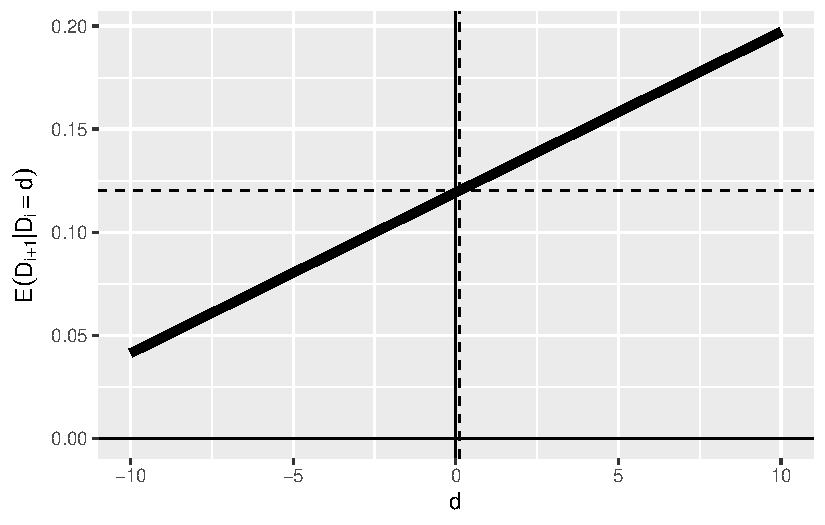
\includegraphics{STAT2857A_examples_23_solutions_files/figure-pdf/unnamed-chunk-3-1.pdf}
\end{center}

Note that when \(d > E(D_i)\) then \(E(D_{i+1}|D_i=d)>E(D_i)\). However,
the increase in \(E(D_{i+1}|D_i=d)\) is much smaller than \(d-E(D_i)\)
because the correlation is so small. In the case that \(d=5\) euros on
one day, the conditional mean is \[
0.1193 + 0.0078 (5) = 0.1583
\] euros so that \[
D_{i+1}|D_i \sim \mbox{Normal}(0.1583, 5.2823).
\] Note that the conditional mean is bigger than the unconditional mean.
Knowning that the stock price increased by 5 euros on one day has
increased the expected stock price on the following day. However, the
gain is relatively minimal.

\begin{enumerate}
\def\labelenumi{\alph{enumi})}
\setcounter{enumi}{1}
\tightlist
\item
  The probability that the price on day \(i+1\) increases given that the
  change on day \(i\) is \(d\) is \[
  P(D_{i+1}>0|D_i=d)
  =\int_0^\infty f_{D_{i+1}|D_i}(x|d)~x.
  \] Alternatively, we can standardize so that \[
  P(D_{i+1}>0|D_i=d)
  =P\left(Z > \frac{-(0.1193 + 0.0078 (5))}{5.2823}\right)
  \] where \(Z\) is standard normal. However, neither of the has an
  analytical solution (i.e., we can't do the integral by hand). Instead,
  we can use the calculator to compute the probability for different
  values of \(d\). The following plot displays the probability that the
  increase is positive on day \(i+1\) given the change on day \(i\). The
  dotted line is the probability that the price increases on a randomly
  selected day.
\end{enumerate}

\begin{center}
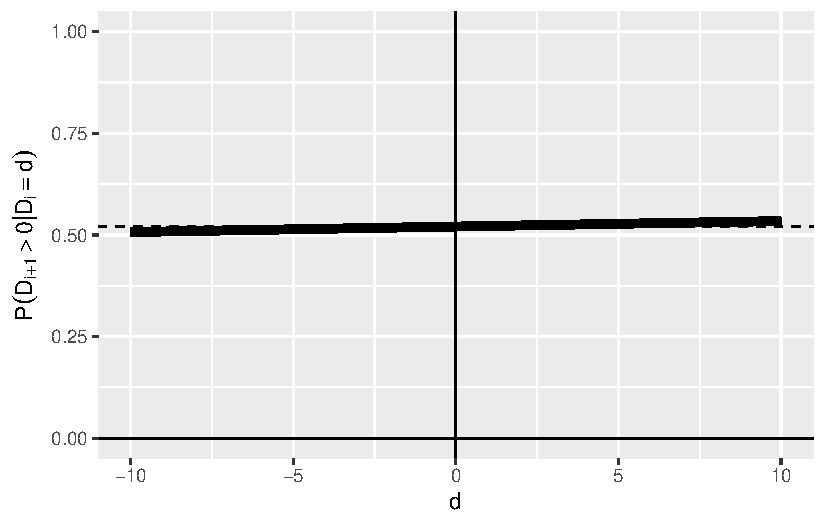
\includegraphics{STAT2857A_examples_23_solutions_files/figure-pdf/unnamed-chunk-4-1.pdf}
\end{center}

To make this clearer, the following plot zooms the \(y\)-axis to the
range \((.4,.6)\).

\begin{center}
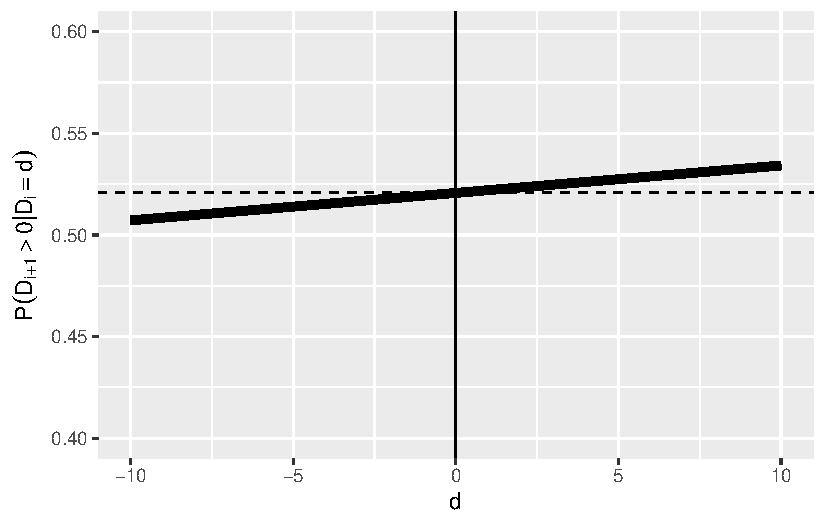
\includegraphics{STAT2857A_examples_23_solutions_files/figure-pdf/unnamed-chunk-5-1.pdf}
\end{center}

You can see that the conditional probability is above marginal
probability when \(d>E(D_i)=0.1202\). However, there isn't much gain.
Given that \(D_i=5\), the probability of an increase on the next day is
only \[
P(D_{i+1}>0|D_i=5)=0.5274.
\] Again, this is an increase from the marginal probability. We have
learned something about \(D_{i+1}\) by observing that \(D_{i}=5\), but
not very much.

\begin{enumerate}
\def\labelenumi{\alph{enumi})}
\setcounter{enumi}{2}
\item
  \begin{enumerate}
  \def\labelenumii{\roman{enumii})}
  \item
    Suppose that the stock price increases by exactly \(d\) euros on
    days \(t_1,\ldots,t_{10}\). The expected gain over all 10 days is \[
    \begin{aligned}
    E\left(\sum_{i=1}^{10}D_{t_i+1}|D_{t_i}=d\right)
    &=\sum_{i=1}^{10} E(D_{t_i+1}|D_{t_i}=d)\\
    &=\sum_{i=1}^{10} 0.1193 + 0.0078d\\
    &=10(0.1193 + 0.0078d).
    \end{aligned}
    \] If \(d=5\), then \[
    E\left(\sum_{i=1}^{10}D_{t_i+1}|D_{t_i}=5\right)
    =1.5826.
    \]
  \item
    As before, if \(Y\) represents the number of days on which the price
    increases, then \(Y\) will be binomial. Specifically, \[
    Y \sim \mbox{Binomial}(10,P(D_{i+1}>0|D_i=d)).
    \] For the case \(d=5\), \[
     P(Y>5)
     =\sum_{y=6}^{10} {10 \choose y} 0.5274^y (1 - 0.5274)^{10-y}
     =0.4461.
      \]
  \item
    Similarly, \[
     P(Y<5)
     =\sum_{x=0}^{5} {10 \choose y} 0.5274^y (1 - 0.5274)^{10-y}
     =0.3115.
     \] The probability that the stock price increases on more than have
    the days is larger than it was before. However, the gain is fairly
    small.
  \end{enumerate}
\end{enumerate}




\end{document}
